\documentclass[t]{beamer}
\usetheme[progressbar=frametitle]{metropolis}
\usepackage{appendixnumberbeamer}

\usepackage{booktabs}
\usepackage[scale=2]{ccicons}

\usepackage{graphics,graphicx,amssymb,amsmath,pgf,comment,hyperref}
%\usepackage[xcolor=pst]{pstricks}
\usepackage{array}
\usepackage{pgfshade}
\usepackage[round]{natbib}
\usepackage[absolute,overlay]{textpos}
\usepackage{pifont}
\usepackage{dcolumn}
\usepackage{textpos}
\usepackage{color}					
\usepackage{xcolor,colortbl}
\usepackage{tikz}
\usepackage{bbm}
\usepackage{curves}
\usepackage{mathtools}
\usetikzlibrary{snakes,arrows,positioning}
\def\augie{\fontencoding{T1}\fontfamily{augie}\selectfont}

\usepackage{pgfplots}
\usepgfplotslibrary{dateplot}

\usepackage{xspace}
\newcommand{\themename}{\textbf{\textsc{metropolis}}\xspace}

\setbeamertemplate{caption}{\raggedright\insertcaption\par}
\usetikzlibrary{calc,decorations.pathmorphing,patterns}
\pgfdeclaredecoration{penciline}{initial}{
    \state{initial}[width=+\pgfdecoratedinputsegmentremainingdistance,
    auto corner on length=1mm,]{
        \pgfpathcurveto%
        {% From
            \pgfqpoint{\pgfdecoratedinputsegmentremainingdistance}
                      {\pgfdecorationsegmentamplitude}
        }
        {%  Control 1
        \pgfmathrand
        \pgfpointadd{\pgfqpoint{\pgfdecoratedinputsegmentremainingdistance}{0pt}}
                    {\pgfqpoint{-\pgfdecorationsegmentaspect
                     \pgfdecoratedinputsegmentremainingdistance}%
                               {\pgfmathresult\pgfdecorationsegmentamplitude}
                    }
        }
        {%TO
        \pgfpointadd{\pgfpointdecoratedinputsegmentlast}{\pgfpoint{1pt}{1pt}}
        }
    }
    \state{final}{}
}


\title{The Effects of Financial Integration with Hospitals on Physician Behaviors}
\date{ASHEcon 2018, Emory University}
\author{Haizhen Lin \& \textbf{Ian McCarthy} \& Michael Richards}
\institute{June 11, 2018}

\begin{document}

\maketitle

\section{Motivation}

\begin{frame}{How are hospitals and physicians related?}
    \only<1>{
        \begin{enumerate}
            \item ``Traditional'' private practice with admitting privileges
            \item Administrative support with or without admitting restrictions
            \item Practice owned by hospital or hospital system
        \end{enumerate}
    }
    \only<2>{
        \begin{figure}
            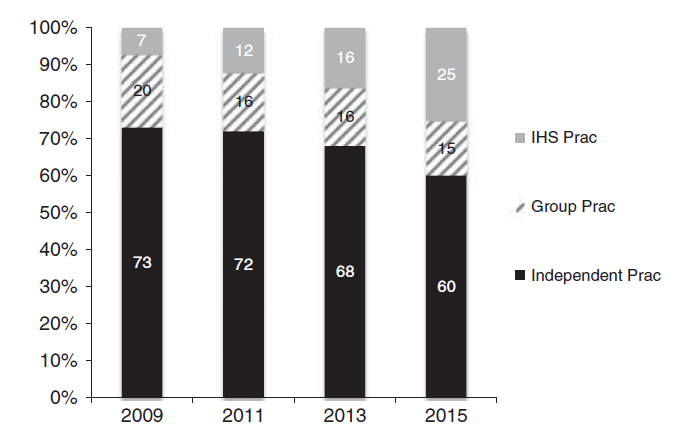
\includegraphics[height=2.4in,keepaspectratio]{Richardsetal.png}
            \caption{Richards \textit{et al.}, Medical Care, 2016}
        \end{figure}
    }
    \only<3>{
        \begin{figure}
            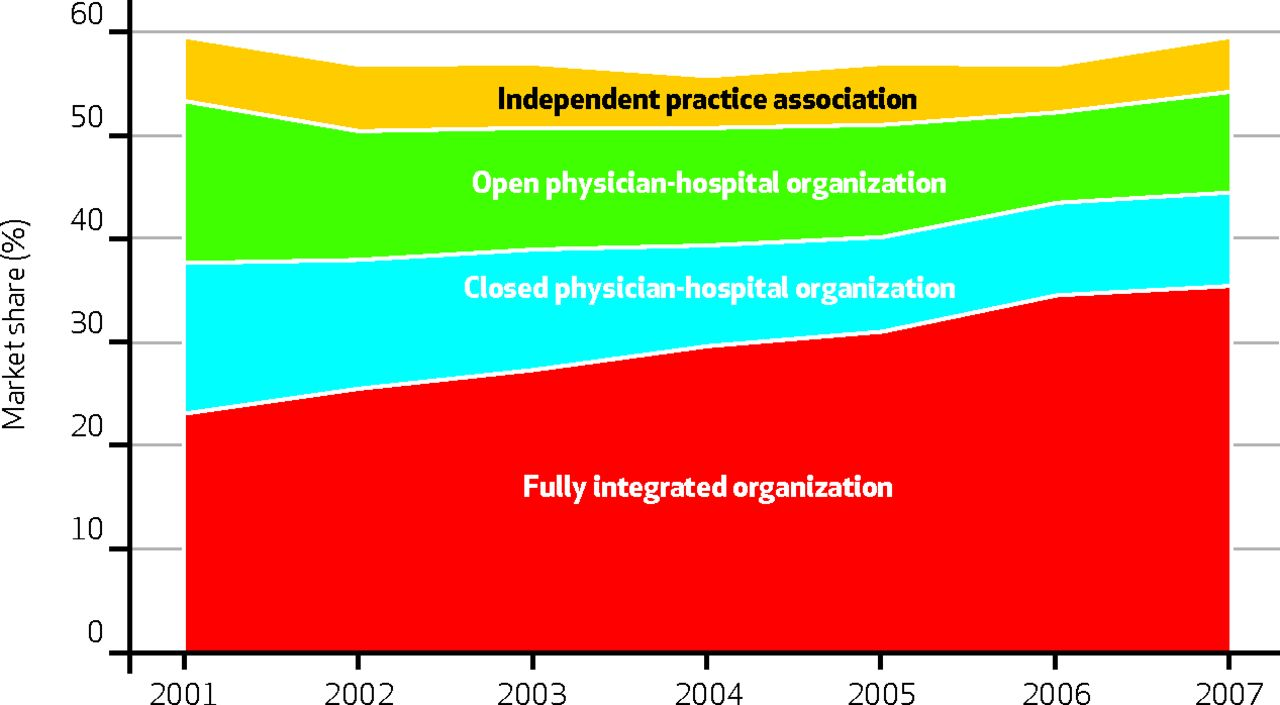
\includegraphics[height=2.3in,keepaspectratio]{Bakeretal.jpg}
            \caption{Baker, Bundorf, and Kessler, Health Affairs, 2014}
        \end{figure}
    }
\end{frame}

\begin{frame}{Why would a hospital integrate?}
    \only<1>{
        \metroset{block=fill}
        \begin{block}{Revenue}
            \begin{itemize}
                \item Increase bargaining position
                \item Bundle products
                \item Exploit payment differentials
            \end{itemize}
        \end{block}
    }

    \only<2>{
        \metroset{block=fill}
        \begin{block}{CMS Incentives}
            \begin{itemize}
                \item Hospital Readmission Reduction Program
                \item Hospital Value Based Purchasing Program
                \item Accountable Care Organizations
                \item Bundled Payments
            \end{itemize}
        \end{block}
    }

    \only<3>{
        \metroset{block=fill}
        \begin{block}{Coordination}
            \begin{itemize}
                \item Remove inefficiencies from fragmented care
                \item Improve quality via ``team-based'' care
            \end{itemize}
        \end{block}
    }
\end{frame}

\begin{frame}{Why would a physician practice integrate?}
    \only<1>{
        \metroset{block=fill}
        \begin{block}{Financial security}
            \begin{itemize}
                \item Salaried arrangement
                \item Potential volume incentives
            \end{itemize}
        \end{block}
    }

    \only<2>{
        \metroset{block=fill}
        \begin{block}{Reduce administrative burden}
            \begin{itemize}
                \item Billing and insurance approvals
                \item Electronic Health Records
                \item Data collection/reporting
            \end{itemize}
        \end{block}
    }
\end{frame}

\begin{frame}{Anticipated effects on physicians}
    \begin{enumerate}
        \item Focus on patient care
        \item Less autonomy
        \item More processes, checklists, etc.
    \end{enumerate}
\end{frame}


\section{Data}
\begin{frame}{Data Sources}
    \begin{itemize}
        \item<1-> CMS: 100\% Medicare claims data (2008-2015)
        \item<2-> SK\&A: Hospital ownership of physician practices
        \item<3-> AHA, HCRIS, POS: Hospital characteristics
        \item<4-> ACS: County-level demographics, education, income, and employment
    \end{itemize}
\end{frame}

\begin{frame}{Sample Construction}
    \begin{itemize}
        \item<1-> Planned inpatient operations with observed NPI for the operating physician, defined as elective admissions initiated by a physician, clinic, or HMO referral
        \item<2-> Drop physicians operating in hospitals more than 120 miles from primary office or outside of contiguous U.S.
        \item<3-> Drop physicians with NPIs not matched in the SK\&A data
        \item<4-> Require at least 15 operations in a given hospital/year
        \item<5-> Balanced panel of physicians from 2008 through 2015
    \end{itemize}
  \uncover<6->{ $\Longrightarrow$ 63,532 unique observations at the physician/hospital/year \\
   $\Longrightarrow$ 3.9mm inpatient stays}
\end{frame}


\section{Empirical Approach}

\begin{frame}{Initial Specification}
    \begin{equation*}
        y_{jht} = \delta_{1} I_{jht} + \delta_{2} I_{ht} + \delta_{3} I_{jt} + \beta_{1} x_{jt} + \beta_{2} z_{ht} + \beta_{3} w_{mt} + \Theta_{jhmt} + \varepsilon_{jht}
    \end{equation*}
\end{frame}


\begin{frame}{Physician Affiliation Outcomes}
    \begin{equation*}
        \textcolor{red}{y_{jht}} = \delta_{1} I_{jht} + \delta_{2} I_{ht} + \delta_{3} I_{jt} + \beta_{1} x_{jt} + \beta_{2} z_{ht} + \beta_{3} w_{mt} + \Theta_{jhmt} + \varepsilon_{jht}
    \end{equation*}

    \begin{table}[htb!]
    \centering
    \footnotesize
    \centerline{
    \begin{tabular}{l|rrrrr|r}
        & 2008  & 2012 & 2013 & 2014 & 2015 & Overall \\
        \hline
Hospital Share&       0.864       &       0.878         &       0.882         &       0.884         &       0.909         &       0.879         \\
              &     (0.225)       &     (0.217)         &     (0.216)         &     (0.215)         &     (0.184)         &     (0.216)         \onslide<2->{ \\
Operations    &       60.80       &       62.16         &       62.02         &       60.45         &       61.68         &       61.64         \\
              &     (43.50)       &     (43.90)         &     (45.08)         &     (45.10)         &     (45.95)         &     (44.45)         }\\
        \end{tabular}}
    \end{table}
\end{frame}

\begin{frame}{Mortality Outcomes}
    \begin{equation*}
        \textcolor{red}{y_{jht}} = \delta_{1} I_{jht} + \delta_{2} I_{ht} + \delta_{3} I_{jt} + \beta_{1} x_{jt} + \beta_{2} z_{ht} + \beta_{3} w_{mt} + \Theta_{jhmt} + \varepsilon_{jht}
    \end{equation*}

    \begin{table}[htb!]
    \centering
    \footnotesize
    \centerline{
    \begin{tabular}{l|rrrrr|r}
        & 2008  & 2012 & 2013 & 2014 & 2015 & Overall \\
        \hline
90-day Mortality &      0.0290     &      0.0260         &      0.0250         &      0.0246         &      0.0252         &      0.0263     \\
                 &    (0.0404)     &    (0.0385)         &    (0.0380)         &    (0.0377)         &    (0.0416)         &    (0.0391)         \onslide<2->{    \\
60-day Mortality &      0.0237     &      0.0211         &      0.0204         &      0.0203         &      0.0200         &      0.0214         \\
                 &    (0.0350)     &    (0.0334)         &    (0.0329)         &    (0.0328)         &    (0.0358)         &    (0.0340)         \onslide<3->{ \\
30-day Mortality &      0.0173     &      0.0152         &      0.0144         &      0.0144         &      0.0140         &      0.0153        \\
                 &    (0.0286)     &    (0.0271)         &    (0.0264)         &    (0.0260)         &    (0.0285)         &    (0.0273)   }}
    \end{tabular}}
    \end{table}
\end{frame}

\begin{frame}{Spending and Treatment Intensity Outcomes}
    \begin{equation*}
        \textcolor{red}{y_{jht}} = \delta_{1} I_{jht} + \delta_{2} I_{ht} + \delta_{3} I_{jt} + \beta_{1} x_{jt} + \beta_{2} z_{ht} + \beta_{3} w_{mt} + \Theta_{jhmt} + \varepsilon_{jht}
    \end{equation*}

    \begin{table}[htb!]
    \centering
    \footnotesize
    \centerline{
    \begin{tabular}{l|rrrrr|r}
        & 2008  & 2012 & 2013 & 2014 & 2015 & Overall \\
        \hline
Payment &     14151.7      &     16237.5         &     16593.1         &     16789.4         &     16796.3         &     15792.2         \\
        &    (6189.7)      &    (7229.5)         &    (7295.5)         &    (7368.5)         &    (7541.3)         &    (7010.4)        \onslide<2->{ \\
Charge  &     50003.6     &     64441.6         &     68092.6         &     71636.7         &     73732.0         &     62436.8         \\
        &   (25952.6)     &   (35412.6)         &   (38170.0)         &   (41206.7)         &   (42881.0)         &   (35694.8)       \onslide<3->{  \\
DRG     &       2.377     &       2.539         &       2.572         &       2.698         &       2.689         &       2.529         \\
        &     (0.764)     &     (0.777)         &     (0.776)         &     (0.917)         &     (0.937)         &     (0.818)       \onslide<4->{  \\
LOS     &       5.659     &       5.620         &       5.560         &       5.644         &       5.624         &       5.572         \\
        &     (1.578)     &     (1.869)         &     (1.894)         &     (2.017)         &     (2.075)         &     (1.783)       }}}
    \end{tabular}}
    \end{table}
\end{frame}


\begin{frame}{Main Independent Variables}
    \begin{equation*}
        y_{jht} = \delta_{1} \textcolor{red}{I_{jht}} + \delta_{2} \textcolor{red}{I_{ht}} + \delta_{3} \textcolor{red}{I_{jt}} + \beta_{1} x_{jt} + \beta_{2} z_{ht} + \beta_{3} w_{mt} + \Theta_{jhmt} + \varepsilon_{jht}
    \end{equation*}

    \begin{table}[htb!]
    \centering
    \footnotesize
    \centerline{
    \begin{tabular}{l|rrrrr|r}
        & 2008  & 2012 & 2013 & 2014 & 2015 & Overall \\
        \hline
$I_{jht}$  &   0.152         &       0.209         &       0.237         &       0.249         &       0.333         &       0.210  \onslide<2->{       \\
$I_{ht}$   &   0.507         &       0.576         &       0.601         &       0.654         &       0.749         &       0.585      \onslide<3->{   \\
$I_{jt}$   &   0.310         &       0.328         &       0.450         &       0.432         &       0.542         &       0.372       }}
        \end{tabular}}
    \end{table}
\end{frame}

\begin{frame}{Risk adjustment and physician-hospital ``match values''}
    \only<1>{
        \begin{itemize}
            \item Isolate variation from physician-hospital interaction
            \item Adjust for patient characteristics
        \end{itemize}
    }
    \only<2-4>{
        \metroset{block=fill}
        \begin{block}{1. Estimate $\gamma_{jh}$}
            \begin{equation*}
                y_{ijh} = \gamma_{j} + \gamma_{jh} + \beta x_{ih} + \varepsilon_{jht}
            \end{equation*}
        \end{block}
    }
    \only<3-4>{
        \metroset{block=fill}
        \begin{block}{2. Use $\hat{\gamma}_{jh}$ as outcome}
            \begin{equation*}
                \underbrace{y_{jht}}_{\hat{\gamma}_{jh}} = \delta_{1} I_{jht} + \delta_{2} I_{ht} + \delta_{3} I_{jt} + \beta_{1} x_{jt} + \beta_{2} z_{ht} + \beta_{3} w_{mt} + \Theta_{jhmt} + \varepsilon_{jht}
            \end{equation*}
        \end{block}
    }
    \only<4>{
        \begin{itemize}
            \item Combined $\gamma_{j} + \gamma_{jh}$ from full sample
            \item Separately identify $\gamma_{jh}$ from physician ``movers''
        \end{itemize}
    }
\end{frame}

\begin{frame}{Endogeneity of physician-hospital integration}
    \only<1>{
        Integration could be driven by:
        \begin{itemize}
            \item Existing physician behaviors
            \item Unobserved, time-varying practice characteristics
        \end{itemize}
    }
    \only<2>{
        \metroset{block=fill}
        \begin{block}{1. Set of possible physician-hospital pairs}
            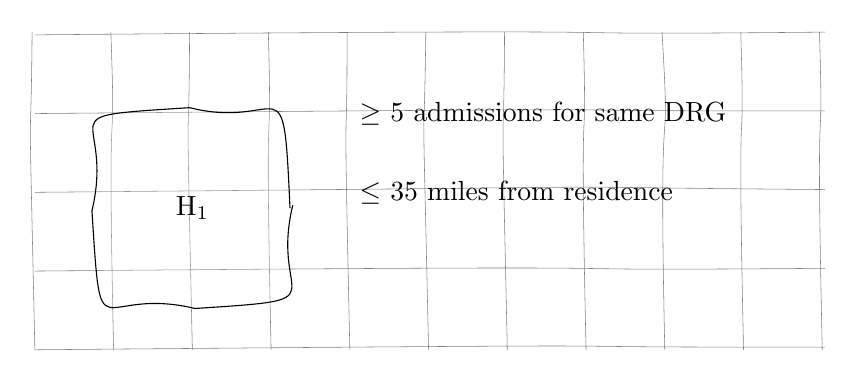
\begin{tikzpicture}[decoration=penciline, decorate]
                \draw[decorate,style=help lines] (0,0) grid[step=1cm] (10,4);

                % Patient 1
                \node[decorate,draw,inner sep=.7cm,fill=white,fill opacity=.2,text opacity=1,circle] (a) at (2,1.8) {$\text{H}_{1}$};

                \node[right] at (4,3) {$\geq$ 5 admissions for same DRG};
                \node[right] at (4,2) {$\leq$ 35 miles from residence};
            \end{tikzpicture}
        \end{block}
    }
    \only<3>{
        \metroset{block=fill}
        \begin{block}{1. Set of possible physician-hospital pairs}
            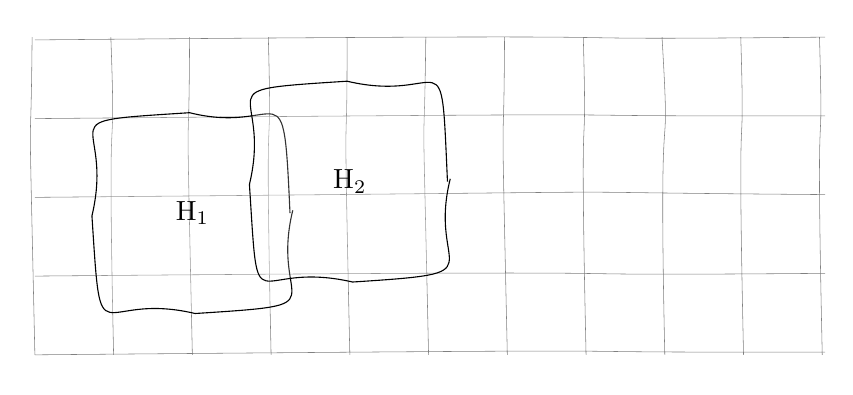
\begin{tikzpicture}[decoration=penciline, decorate]
                \draw[decorate,style=help lines] (0,0) grid[step=1cm] (10,4);

                % Patient 1
                \node[decorate,draw,inner sep=.7cm,fill=white,fill opacity=.2,text opacity=1,circle] (a) at (2,1.8) {$\text{H}_{1}$};

                % Patient 2
                \node[decorate,draw,inner sep=.7cm,fill=white,fill opacity=.2,text opacity=1,circle] (a) at (4,2.2) {$\text{H}_{2}$};

            \end{tikzpicture}
        \end{block}
    }
    \only<4>{
        \metroset{block=fill}
        \begin{block}{1. Set of possible physician-hospital pairs}
            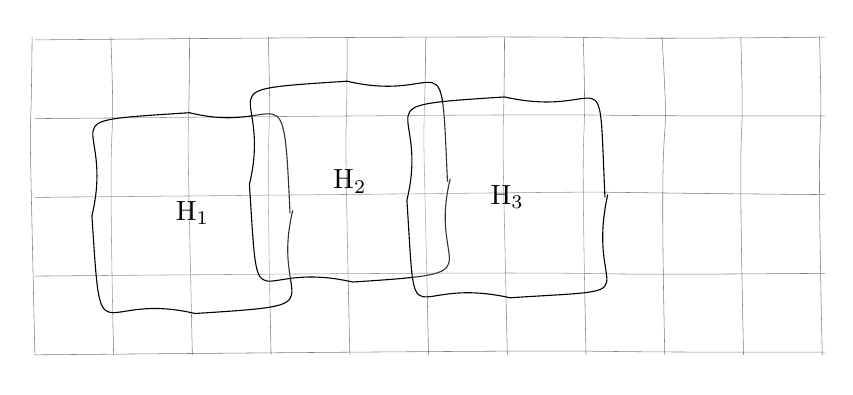
\begin{tikzpicture}[decoration=penciline, decorate]
                \draw[decorate,style=help lines] (0,0) grid[step=1cm] (10,4);

                % Patient 1
                \node[decorate,draw,inner sep=.7cm,fill=white,fill opacity=.2,text opacity=1,circle] (a) at (2,1.8) {$\text{H}_{1}$};

                % Patient 2
                \node[decorate,draw,inner sep=.7cm,fill=white,fill opacity=.2,text opacity=1,circle] (a) at (4,2.2) {$\text{H}_{2}$};

                % Patient 3
                \node[decorate,draw,inner sep=.7cm,fill=white,fill opacity=.2,text opacity=1,circle] (a) at (6,2) {$\text{H}_{3}$};

            \end{tikzpicture}
        \end{block}
    }
    \only<5>{
        \metroset{block=fill}
        \begin{block}{1. Set of possible physician-hospital pairs}
            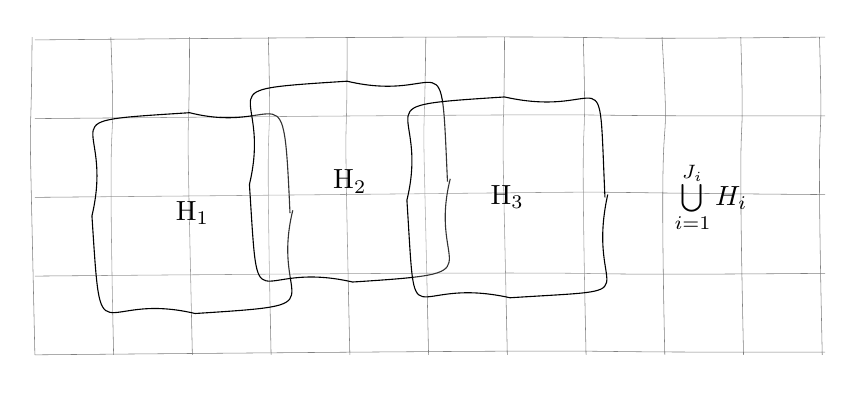
\begin{tikzpicture}[decoration=penciline, decorate]
                \draw[decorate,style=help lines] (0,0) grid[step=1cm] (10,4);

                % Patient 1
                \node[decorate,draw,inner sep=.7cm,fill=white,fill opacity=.2,text opacity=1,circle] (a) at (2,1.8) {$\text{H}_{1}$};

                % Patient 2
                \node[decorate,draw,inner sep=.7cm,fill=white,fill opacity=.2,text opacity=1,circle] (a) at (4,2.2) {$\text{H}_{2}$};

                % Patient 3
                \node[decorate,draw,inner sep=.7cm,fill=white,fill opacity=.2,text opacity=1,circle] (a) at (6,2) {$\text{H}_{3}$};

                \node[right] at (8,2) {$\bigcup\limits_{i=1}^{J_{i}} H_{i}$};
            \end{tikzpicture}
        \end{block}
    }
    \only<6>{
        \metroset{block=fill}
        \begin{block}{2. Estimate probability of integration}
            \begin{equation*}
                I_{ph} = \lambda_{1} z_{h} + \lambda_{2} z_{ph} + \omega_{ph}
            \end{equation*}
            \vspace{-.3in}
            \begin{itemize}
                \item Average choice set size
                \item Average differential distance (relative to nearest hospital)
            \end{itemize}
        \end{block}
    }
    \only<7>{
        \metroset{block=fill}
        \begin{block}{2. Estimate probability of integration}
            \begin{equation*}
                I_{ph} = \lambda_{1} z_{h} + \lambda_{2} z_{ph} + \omega_{ph}
            \end{equation*}
            \vspace{-.3in}
            \begin{itemize}
                \item Average choice set size
                \item Average differential distance (relative to nearest hospital)
            \end{itemize}
        \end{block}
        \begin{equation*}
            y_{jht} = \delta_{1} \underbrace{I_{jht}}_{\mathclap{\hat{I}_{jht}=\text{Pr}(I_{jht}=1)}} + \delta_{2} I_{ht} + \delta_{3} I_{jt} + \beta_{1} x_{jt} + \beta_{2} z_{ht} + \beta_{3} w_{mt} + \Theta_{jhmt} + \varepsilon_{jht}
        \end{equation*}
    }
\end{frame}

\section{Results}
\begin{frame}{Integration and physician affiliation}
    \only<1>{
    \begin{columns}
        \begin{column}{.6\textwidth}
            \textbf{Fixed Effects Estimator}
            \vspace{.045in}
            \begin{table}[htb!]
            \centering
            \footnotesize
            \centerline{
            \begin{tabular}{l|rr}
                            &  Hospital Share & Operations   \\
                \hline
                $I_{jht}$   &       0.046***&       4.574*** \\
                            &     (0.004)   &     (0.510)    \\
                $I_{ht}$    &       0.005***&       0.670*** \\
                            &     (0.002)   &     (0.232)    \\
                 $I_{jt}$   &      -0.012***&      -1.127*** \\
                            &     (0.002)   &     (0.285)    \\
                \hline
                Net          &    0.0392***  &     4.1180***    \\
                             &   (0.0036)    &     (0.4394)     \\
                \hline
                \multicolumn{3}{l}{* p$<$0.1, ** p$<$0.05, *** p$<$0.01}
            \end{tabular}}
            \end{table}
        \end{column}
        \begin{column}{.4\textwidth}
        \end{column}
    \end{columns}
    }
    \only<2>{
    \begin{columns}
        \begin{column}{.6\textwidth}
            \textbf{Fixed Effects Estimator}
            \vspace{.045in}
            \begin{table}[htb!]
            \centering
            \footnotesize
            \centerline{
            \begin{tabular}{l|rr}
                            &  Hospital Share & Operations   \\
                \hline
                $I_{jht}$   &       0.046***&       4.574*** \\
                            &     (0.004)   &     (0.510)    \\
                $I_{ht}$    &       0.005***&       0.670*** \\
                            &     (0.002)   &     (0.232)    \\
                 $I_{jt}$   &      -0.012***&      -1.127*** \\
                            &     (0.002)   &     (0.285)    \\
                \hline
                Net          &    0.0392***  &     4.1180***    \\
                             &   (0.0036)    &     (0.4394)     \\
                \hline
                \multicolumn{3}{l}{* p$<$0.1, ** p$<$0.05, *** p$<$0.01}
            \end{tabular}}
            \end{table}
        \end{column}
        \begin{column}{.4\textwidth}
            \textbf{With Instrument, $\hat{I}_{jht}$}
            \begin{table}[htb!]
            \centering
            \footnotesize
            \centerline{
            \begin{tabular}{|rr}
                  Hospital Share & Operations   \\
                \hline
                       0.072***&      11.885*** \\
                     (0.017)   &     (4.170)    \\
                       0.004** &       0.489*   \\
                     (0.002)   &     (0.256)    \\
                      -0.019***&      -3.175*** \\
                     (0.005)   &     (1.223)    \\
                \hline
                    0.0573***  &     9.1988***    \\
                   (0.0119)    &     (2.8800)     \\
            \end{tabular}}
            \end{table}
        \end{column}
    \end{columns}
    }
\end{frame}


\begin{frame}{Integration and mortality}
    \only<1-3>{
    \begin{columns}
        \begin{column}{.6\textwidth}
            \textbf{Fixed Effects Estimator}
            \vspace{.045in}
            \begin{table}[htb!]
            \centering
            \scriptsize
            \centerline{
            \begin{tabular}{l|rrr}
                            &  90-day & 60-day & 30-day   \\
                \hline
                Overall     &     0.0016**  &     0.0010   &      0.0009  \\
                            &   (0.0008)    &    (0.0007)  &     (0.0006)  \onslide<2->{\\
                Match Value &     0.0011    &     0.0006   &      0.0010   \\
                            &   (0.0009)    &    (0.0008)  &     (0.0006)  \onslide<3->{\\
                ``Movers''  &     0.0042    &     0.0037   &      0.0008   \\
                            &   (0.0034)    &    (0.0029)  &     (0.0024)  }}\\
                \hline
                \multicolumn{4}{l}{* p$<$0.1, ** p$<$0.05, *** p$<$0.01}
            \end{tabular}}
            \end{table}
        \end{column}
        \begin{column}{.4\textwidth}
        \end{column}
    \end{columns}
    }
    \only<4-6>{
    \begin{columns}
        \begin{column}{.6\textwidth}
            \textbf{Fixed Effects Estimator}
            \vspace{.045in}
            \begin{table}[htb!]
            \centering
            \scriptsize
            \centerline{
            \begin{tabular}{l|rrr}
                            &  90-day & 60-day & 30-day   \\
                \hline
                Overall     &     0.0016**  &     0.0010   &      0.0009  \\
                            &   (0.0008)    &    (0.0007)  &     (0.0006)   \\
                Match Value &     0.0011    &     0.0006   &      0.0010   \\
                            &   (0.0009)    &    (0.0008)  &     (0.0006) \\
                ``Movers''  &     0.0042    &     0.0037   &      0.0008   \\
                            &   (0.0034)    &    (0.0029)  &     (0.0024)  \\
                \hline
                \multicolumn{4}{l}{* p$<$0.1, ** p$<$0.05, *** p$<$0.01}
            \end{tabular}}
            \end{table}
        \end{column}
        \begin{column}{.4\textwidth}
            \textbf{With Instrument, $\hat{I}_{jht}$}
            \begin{table}[htb!]
            \centering
            \scriptsize
            \centerline{
            \begin{tabular}{|rrr}
                              90-day & 60-day & 30-day   \\
                \hline
                          0.0030   &     0.0014   &      0.0010  \\
                        (0.0022)   &    (0.0019)  &     (0.0016)  \onslide<5->{\\
                         0.0012    &     0.0001   &      0.0023   \\
                       (0.0023)    &    (0.0021)  &     (0.0018)   \onslide<6->{\\
                         0.0041    &     0.0028   &      0.0071   \\
                       (0.0296)    &    (0.0272)  &     (0.0212)  }}\\
            \end{tabular}}
            \end{table}
        \end{column}
    \end{columns}
    }
\end{frame}


\begin{frame}{Integration and spending/treatment}
    \only<1-3>{
    \begin{columns}
        \begin{column}{.6\textwidth}
            \textbf{Fixed Effects Estimator}
            \vspace{.045in}
            \begin{table}[htb!]
            \centering
            \scriptsize
            \centerline{
            \begin{tabular}{l|rrr}
                            &  Payment & Charge & DRG  \\
                \hline
                Overall    &  245***  &   3,076***  &    0.0369***  \\
                           &   (71.33)   &   (450)    &    (0.0091)  \onslide<2->{\\
                Match Value &    102   &   2,094***  &    0.0197**   \\
                            &   (68.26)   &   (452)    &     (0.008)   \onslide<3->{\\
                ``Movers''  &    201   &   2,086**  &    0.0642**   \\
                            &   (245.97)  &   (1,217)  &    (0.0276)   }}\\
                \hline
                \multicolumn{4}{l}{* p$<$0.1, ** p$<$0.05, *** p$<$0.01}
            \end{tabular}}
            \end{table}
        \end{column}
        \begin{column}{.4\textwidth}
        \end{column}
    \end{columns}
    }
    \only<4-6>{
    \begin{columns}
        \begin{column}{.6\textwidth}
            \textbf{Fixed Effects Estimator}
            \vspace{.045in}
            \begin{table}[htb!]
            \centering
            \scriptsize
            \centerline{
            \begin{tabular}{l|rrr}
                            &  Payment & Charge & DRG  \\
                \hline
                Overall    &  245***  &   3,076***  &    0.0369***  \\
                           &   (71.33)   &   (450)    &    (0.0091) \\
                Match Value &    102   &   2,094***  &    0.0197**   \\
                            &   (68.26)   &   (452)    &     (0.008) \\
                ``Movers''  &    201   &   2,086**  &    0.0642**   \\
                            &   (245.97)  &   (1,217)  &    (0.0276)   \\
                \hline
                \multicolumn{4}{l}{* p$<$0.1, ** p$<$0.05, *** p$<$0.01}
            \end{tabular}}
            \end{table}
        \end{column}
        \begin{column}{.4\textwidth}
            \textbf{With Instrument, $\hat{I}_{jht}$}
            \begin{table}[htb!]
            \centering
            \scriptsize
            \centerline{
            \begin{tabular}{|rrr}
                              Payment & Charge & DRG  \\
                \hline
                          321     &   4,415***  &    0.0392    \\
                          (267.62)   &   (1,625)   &   (0.0340)   \onslide<5->{\\
                          -588*** &   683     &    -0.0619**   \\
                          (216.77)   & (1,461)    &     (0.0261)   \onslide<6->{\\
                          -1,251   &   -3,564   &    -0.3938*   \\
                          (1,951)  &   (9,141)  &    (0.2316)   }}\\
            \end{tabular}}
            \end{table}
        \end{column}
    \end{columns}
    }
\end{frame}

\begin{frame}{Summary of Results}
    \begin{itemize}
        \item<1-> Increase in shares of 4-6 percentage points (4-9 operations)
        \item<2-> No improvement in mortality
        \item<3-> Evidence that integration changes both coding behaviors (upcoding) and patient selection (healthier patients)
    \end{itemize}
\end{frame}

\end{document}






